

\chapter{Introduction}
\label{chap:Introduction}

\section{NASA Magnetospheric MultiScale Mission}
\label{sec:NASAMagnetosphericMultiScaleMission}

NASA's Magnetospheric MultiScale (MMS) Mission is a Solar Terrestrial probe mission scheduled for launch in October 2014 \cite{mms_website}.  The mission consists of four identical satellites orbiting the Earth in a constellation formation flight.  Construction of the satellites is occurring at NASA's Goddard Space Flight Center (GSFC) where they are being equipped to study the microphysics of magnetic reconnection events within the Earth's magnetic fields.

\begin{figure}[H]
\centerline{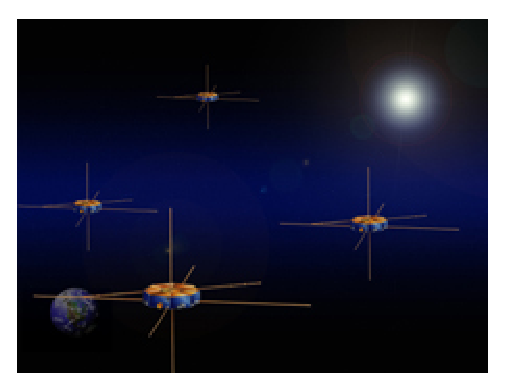
\psfig{file=figures/mms_spacecraft_formation.eps,height=1.2in}}
\caption{MMS Spacecraft Formation}
\label{fig:magneticfields}
\end{figure}

A reconnection event occurs when magnetic field lines cross allowing energetic particles to traverse from interstellar space into the Earth's magnetosphere releasing large quantities of heat and kinetic energy.  The diffusion region of a reconnection event starts on the day side magnetopause an quickly folds over to the Earth's magnetotail (Figure \ref{fig:magneticfields}).  This region is only 1-10 km in size but can travel at 10-100 km/hr \cite{swri} making it extremely difficult to measure.  Effects of a reconnection event are regularly experienced via the aurora borealis, interference with spacecraft GPS systems, and disruptions to electrical grids and communication networks.

\begin{figure}[H]
\centerline{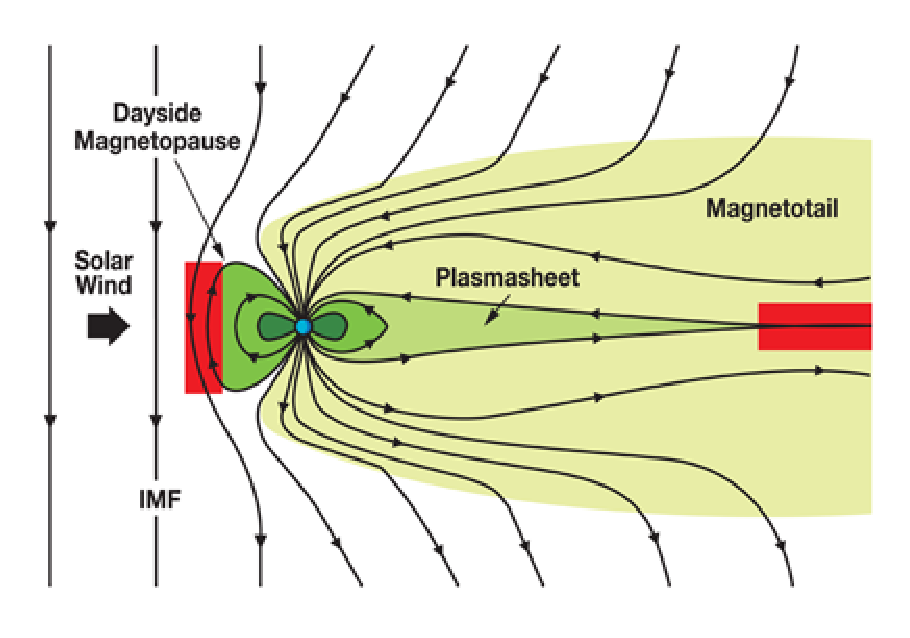
\psfig{file=figures/2d_earth_mag_field_lines.eps,height=1.2in}}
\caption{Earth's magnetic field}
\label{fig:magneticfields}
\end{figure}

Despite the widely experienced effects of reconnection events, very little about the microphysics inside its the diffusion region has been adequately measured.  Magnetometers, spectrometers, and other equipment currently in orbit are only able to capture a small fraction of the event's behavior.  Most equipment collect data from a single point or direction in space or some can get a 360 view of space by applying a slow spin to the spacecraft.  Both of these measurement methods are insufficient at capturing the structure of the diffusion region as it passes.

MMS's four satellites will be equipped with instrumentation mounted at the end of six boom extending out from the spacecraft's body along each major axis.  Four boom are the Spin Plane Double Probes (SDP) and two Axial Double Probes (ADP).  This configuration along with high resolution electron and ion spectrometers gives the constellation a new insight into the internal structure of the diffusion region.  The instrumentation at the ends of the boom are an advantage to the science portion of the mission, but create a unique challenge for the Attitude Determination and Control Systems (ADCS).  The satellites are spin stabilized at a rate of 3 rpm.  Disturbances to the rotation could translate into undesirable boom dynamics and nutations off the spin plane.



% Science questions to answer \cite{mms_website}
%     What determines when reconnection starts and how fast it proceeds?
%     What is the structure of the diffusion region?
%     How do the plasmas and magnetic fields disconnect and reconnect in the diffusion regions?
%     What role do the electrons play in facilitating reconnection?
%     What is the role of turbulence in the reconnection process?
%     How does reconnection lead to the acceleration of particles to high energies?


% \todo{image of formation flight}
% study microphysics of
%   magnetic reconnection
%   energetic particle acceleration
%   turbulence

% s/c MMS-1, MMS-2..MMS-4
% reconnection: Electromagnetic energy from the sun interacts with Earth's magnetosphere causing magnetic field lines to cross and create a burst of energy \cite{nasa_edge_video_ne_at_mms}
% magnetic reconnection measured ions and electrons as boundary passes to create 3d model of it passing by
% Fast plasma investigation
% probing the electron diffusion region (EDR) (passes too rapidly to get an accurate view with current equipment small (1-10 km) and rapidly moving (10-100 km/s))
% adjacent magnetic fields generally have significantly different orientations such that when they intersect, a large amount of energy is dispursed within a small region in the form of heat and kinetic energy.  The region = diffusion region
% explore magnetic reconnection
% dynamic regions of magnetosphere
% orbits planned to pass through the upstream and downstream magnetic reconnection sites
% 1) day side - solar wind field lines connection
% 2) down stream -
% 3) plasma travels down and causes the Arura
% through magnetospheric reconnection, portals allow energetic particles to traverse from outside to the interior of the magnetosphere
% predict when solar space weather within the magnetosphere and if they will affect orbiting satellites
% adverse space weather within the magnetosphere can negatively impact spacecraft system health GPS, induce disruptive current in electrical grids, communications, increased radiation exposure on trans-polar flights

% Difficult to understand
% magnetic boundary passes satellites quickly so has been hard to measure
% MMS has instruments to capture measurements
% Instruments mounted on all sides of the
% 8 sensors 1/30th sec instead of

% October 2014, Atlas five launch \cite{nasa_edge_video}

% Sensors
%   star sensor -> attitude
%   accelerometers -> $\Delta V$


% Fast Plasma Instrument (FPI) - controls
%   16 Dual Electron spectrometer (DES) Goddard built
%   16 Dual Ion Spectrometer (DIS) Japan *** built, hand delivered
%   180 degree and +- 22 degree measurement
%   30 millisec measurement rate 100x faster than previous missions entire view of sky
% FPI
%   despins data

% Instument Data processing Unit (IDPU) - brains of measurements
%   collects, compresses, transmits requested measurement data
%   configure while on mission

% booms
%   eight deployable booms
%   two 12.5m axial booms (electric field sensors)
%   four 60m wire booms
%   two 5m booms in spin plane for magnetometers
% rigid, wire, top/bottom booms
% important to keep consistent spin rate to get accurate estimates of boom location


% \section{Propulsion}

% types: solid propellents, bi propellents, electro propulsion, cold gas systems
% chose: mono-propellant blowdown - hydrozene power thrusters \cite{nasa_edge_video_propulsion}
% 3 rpm
% radial thrusters - spinning
% axial thrusters - prevent nutation

% concern:
% propulsion introduce distrubances

% 20 second pulses

% fuel limits by number of adjustments


% \section{performance requirements}

% $\pm 0.5$ deg attitude tollerance
% 1/10th of a second

\section{Research Objective}
\label{sec:ResearchObjective}

The work described in this thesis utilizes an experimental tabletop satellite (TableSat) \cite{vessthesis} to span three main efforts.  First is to create a physical model of a satellite from NASA's Magnetospheric MultiScale (MMS) Mission in order to validate and compare varied gyroless attitude determination and control (ADC) techniques.  The ADC systems must keep the TableSat rotating at a constant 3 rpm, prevent boom oscillations, and correct for detected nutations off the spin plane.  The second goal is to produce a software system that can be used to run against both theoretical simulations and experimental models.  The third goal is improve TableSat's use as an outreach tool.  The system should provide near ``real-time'' feedback of the system's state, allow for on-the-fly modification to control parameters, and be designed such that a individuals specializing in control systems could customize and extend its functionality without substantial computer science expertise.

\section{Past Work}
\label{sec:PastWork}

This work is a direct extension off of Vess' \cite{vessthesis} research using TableSat through Matlab Simulink and onboard flight controllers to demonstrate fundamentals of control theory.  The TableSat experimental design was modified to study the system dynamics of the instrument booms and nutation actuators in NASA's MMS mission satellites.  Previous experimental \cite{tsat1b} \cite{tsat1c} \cite{tsat2} and analytical \cite{mushawehthesis} ADC work at University of New Hampshire's Advanced Control Lab (ACL) has been done targeting the MMS mission.  The TableSat platform or similar derivations have also been adapted in investigate other areas of research including embedded systems development \cite{tablesat_xuml} and fault tolerant control \cite{tablesat_object_bench} \cite{nanjing_university}.


\section{Analytical and Experimental Testbed}
\label{sec:AnalyticalandExperimentalTestbed}



\section{Thesis Contributions}
\label{sec:ThesisContributions}

This research contributes to the field of feedback control, particularly as it relates to spin stabilized spacecraft, in the following ways:

\begin{itemize}
\item Gyroless observer-based controllers used to detect and eliminate nutations and maintain control of a spin stabilized satellite.
\item Improved capabilities of validating observer-based control methods by keeping identical control systems between analytical simulations and real experiments.
\item Allow clusters of estimators and controllers to all receive the same update for improved side-by-side comparisons of effectiveness.
\item Reduce time required to tune a controller by allowing for gain adjustments and swapping of estimation/control techniques on-the-fly.
\item Decompose quaternion state into separate rotational and nutation quaternions for use in error correction.
\item Use decomposed quaternion and differentiated rotational quaternions to decouple rate and attitude control.
\item Base quaternion state corrections on the representative rotational angle error, not the quaternion's sinusoidal scalar term.
\item Build the application such that the same control laws can be used to drive analytical simulations as well as experimental tests with physical systems.
\item Develop the application in a modular fashion to easily allow for future improvements and additions.
\item Control rates between modules such as sensors to estimators and estimators to controllers are independent and can operate at separate rates.
\item ``run-time'' feedback is available to visualize how the controller believes the system is responding.
\item A global clock instance is used for the authoritative time which during simulations can be adjusted in runtime to speed up or slow down the simulation to obtain better insight into the system dynamics.
\item Compensations for variable step sizes ($\delta t$) are made where able to protect the numerical integrity of the controller under large changes in control rates.
\item Code covered by proper software unit tests to validate and maintain expected behavior of the system during software upgrades.
\item Provide the combination of ``run-time'' visualizations and on-the-fly parameter/controller tuning for outreach programs.
\item Write the control application in a high level language to keep it accessible for improvements to control systems engineers with moderate programming experience.
\end{itemize}

\section{Thesis Outline}
\label{sec:ThesisOutline}


